\documentclass[serif,mathserif]{beamer}
\usepackage{amsmath, amsfonts, epsfig, xspace}
\usepackage{algorithm,algorithmic}
\usepackage{pstricks,pst-node}
\usepackage{multimedia}
\usepackage[normal,tight,center]{subfigure}
\setlength{\subfigcapskip}{-.5em}
\usepackage{beamerthemesplit}
\usetheme{lankton-keynote}

\author[CodeCat v0.1]{ CodeCat manual tool for codereview \quad 
\includegraphics[width=2.5cm]{images/codecat00.png} }

\title[ Page \hspace{2em}\insertframenumber/\inserttotalframenumber]{CodeCat}

\date{November 11, 2019} 

\institute{Antonio Costa - CoolerVoid - coolerlair[aT]gmail[DOt]com}

\begin{document}

\maketitle

% \section{Introduction}  % add these to see outline in slides


\begin{frame}
  \frametitle{Whoami}
  Author:
<<<<<<< HEAD
  \begin{itemize}  \item Antonio Costa "CoolerVoid" just another Computer Programmer.
=======
  \begin{itemize}  \item Antonio Costa "CoolerVoid" an ordinary Developer.
>>>>>>> b70501dd34d9fecdda1ae509a521993ffa88888a
  \end{itemize}
  \begin{figure}[t]
    \centering
    \subfigure[]{
    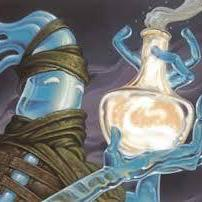
\includegraphics[width=3cm]{images/tony.jpeg}}
  \end{figure}
\end{frame}


\begin{frame}
  \frametitle{Introduction}
  Software Information:
  \begin{itemize}
<<<<<<< HEAD
  \item  CodeCat is a Open Source Tool, your focus is help in codereview. 
=======
  \item  CodeCat is a Open Source Tool, focused to help code review. 
>>>>>>> b70501dd34d9fecdda1ae509a521993ffa88888a
  \item  CodeCat held by GPL v3 license
  \end{itemize}
\end{frame}



\begin{frame}
  \frametitle{Introduction}
  Motivations
  \begin{itemize}
  \item  Track untrusted user input 
  \item  Track dangerous functions
  \item  Save sinks in cache and show syntax highlight to study all codes.
  \item  Options to save custom rule to search new sinks	  
  \end{itemize}
\end{frame}



\begin{frame}
  \frametitle{Introduction}
  Requirements:
  \begin{itemize}
  \item  Python3 
  \item  Current version tested only in Linux.
  \item  Current version run well, but is a BeTa version, you can report bug...
  \end{itemize}
\end{frame}

% \section{Main Body} % add these to see outline in slides

\begin{frame}
  \frametitle{How you can use it}
  Following this to get, decompress and install:
  \begin{itemize}
  \item git clone https://github.com/CoolerVoid/codecat
  \item Follow steps of readme.md file
  \end{itemize}
\end{frame}



\begin{frame}
  \frametitle{The Overview}
  \begin{figure}[]    
    \centering
    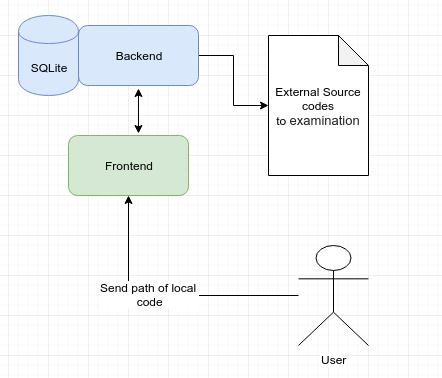
\includegraphics[width=9cm]{images/diagram0.png} 
  \end{figure}
\end{frame}


\begin{frame}
<<<<<<< HEAD
  \frametitle{Explain}
=======
  \frametitle{Explanation}
>>>>>>> b70501dd34d9fecdda1ae509a521993ffa88888a
  Following left menu you have options to custom rules.
  \begin{itemize}
  \item You can create, list, remove your custom rules...
  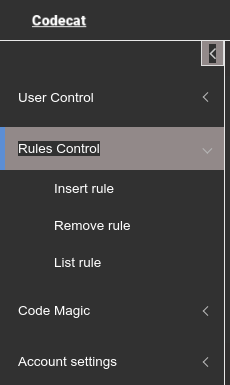
\includegraphics[width=2cm]{images/menu1.png} 
  \end{itemize}
\end{frame}

\begin{frame}
<<<<<<< HEAD
  \frametitle{Explain}
=======
  \frametitle{Explanation}
>>>>>>> b70501dd34d9fecdda1ae509a521993ffa88888a
  Insert your custom rule ex 1
  \begin{itemize}
  \item Example to detect simple XSS 	  
  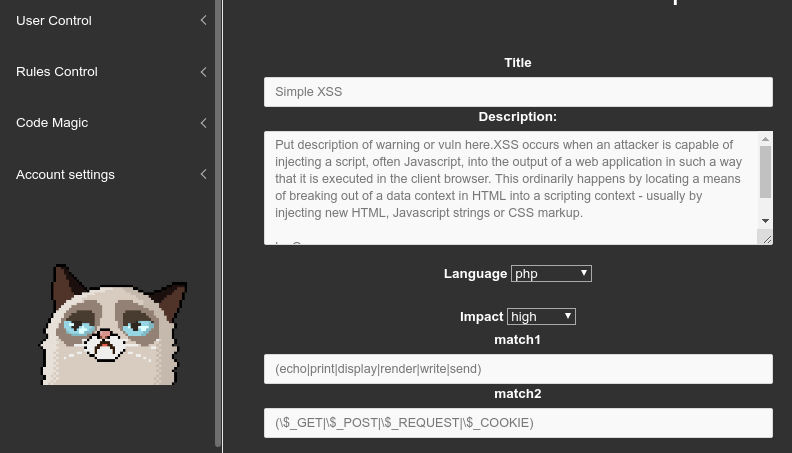
\includegraphics[width=9cm]{images/insertrule2.png} 
  \end{itemize}
\end{frame}

\begin{frame}
<<<<<<< HEAD
  \frametitle{Explain}
=======
  \frametitle{Explanation}
>>>>>>> b70501dd34d9fecdda1ae509a521993ffa88888a
  Insert your custom rule ex 2
  \begin{itemize}
  \item Note, form with value zero, not find match	  
  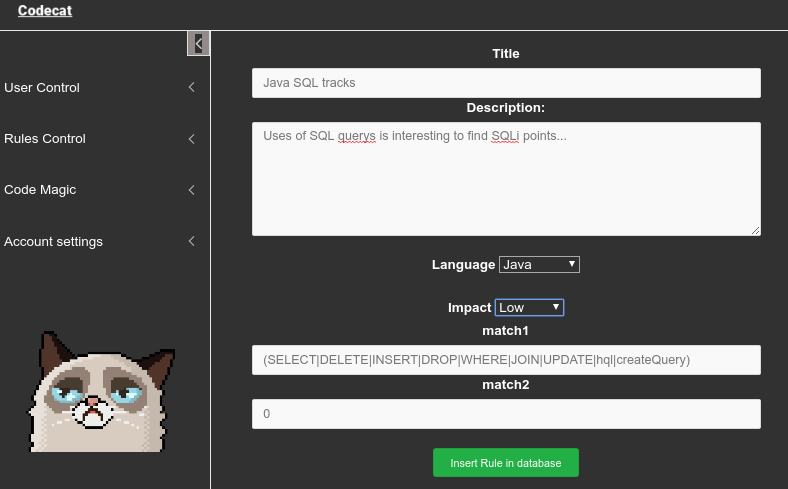
\includegraphics[width=9cm]{images/insertrule.png} 
  \end{itemize}
\end{frame}


\begin{frame}
<<<<<<< HEAD
  \frametitle{Explain}
=======
  \frametitle{Explanation}
>>>>>>> b70501dd34d9fecdda1ae509a521993ffa88888a
  Recursive search by rules in path
  \begin{itemize}	
  \item example from github.com/joostvanveen/php-security-pitfalls
  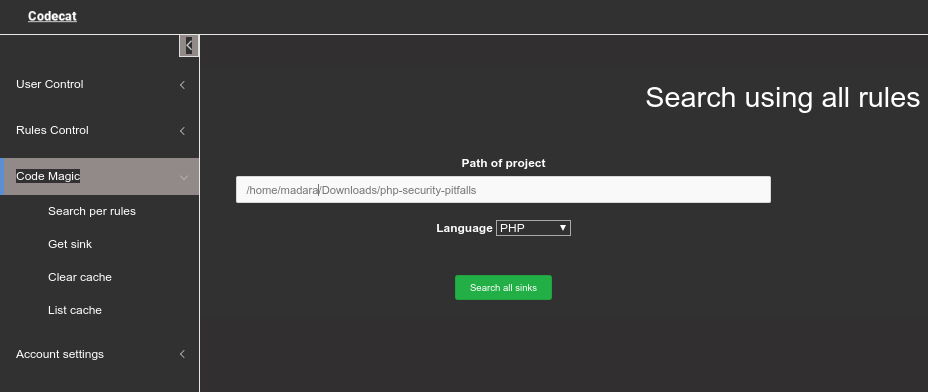
\includegraphics[width=9cm]{images/allsinks.png} 
  \end{itemize}
\end{frame}

\begin{frame}
<<<<<<< HEAD
  \frametitle{Explain}
  You can view the result in cache
=======
  \frametitle{Explanation}
  The results will appear in cache
>>>>>>> b70501dd34d9fecdda1ae509a521993ffa88888a
  \begin{itemize}
  \item If you click in ID Rule you can view rule descriptions...		  
  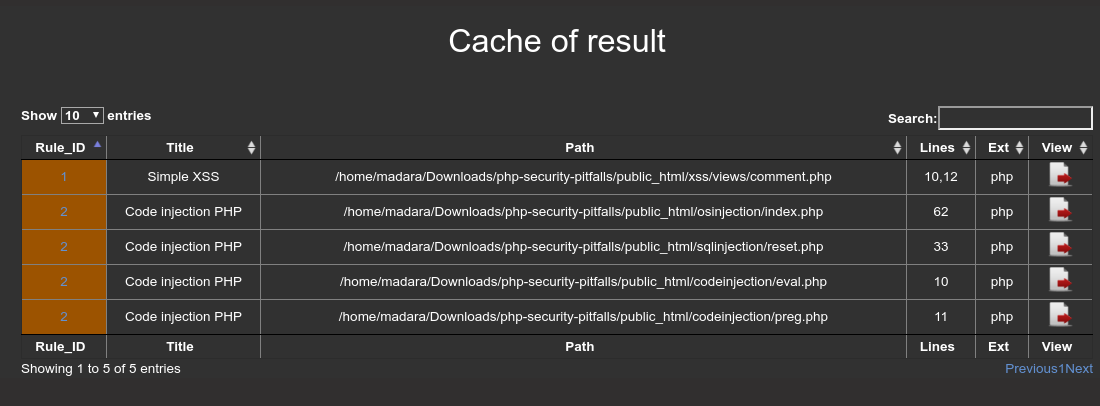
\includegraphics[width=11cm]{images/cache.png} 
  \end{itemize}
\end{frame}


\begin{frame}
<<<<<<< HEAD
  \frametitle{Explain}
=======
  \frametitle{Explanation}
>>>>>>> b70501dd34d9fecdda1ae509a521993ffa88888a
  You can view source of match, when you click view icon
  \begin{itemize}	
  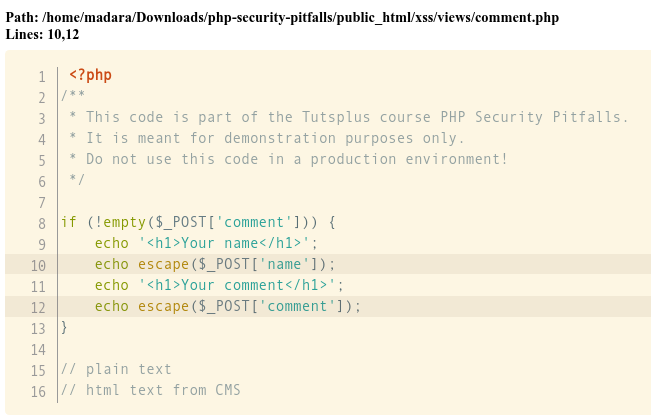
\includegraphics[width=9cm]{images/codeview.png} 
  \end{itemize}
\end{frame}


\begin{frame}
  \frametitle{The End ?}
  \begin{figure}[]    
    \centering
    
\includegraphics[width=5cm]{images/codecat00.png} 
  \end{figure}
\end{frame}



% \section{Conclusion} % add these to see outline in slides

\begin{frame}
  \frametitle{Greets}
  \begin{itemize}
  \item contact: coolerlair[at]gmail[dot]com 
  \item coolerlair[at]gmail[dot]com
  \item my parents and friends...
  \item github.com/CoolerVoid
  \end{itemize}
\end{frame}

\begin{frame}
  \frametitle{at construction...}
\end{frame}

\end{document}

